In cui si spiega nei dettagli lo sviluppo del frontend web facente veci di SPA.

\section{Client API}
Per questo componente un pezzo chiave è il client API. Nuxt offre diversi pattern, architetture e librerie per lo scopo.

\subsection{Prefisso}
Il file di configurazione di Nuxt (\texttt{nuxt.config.ts} \cite{nuxt-config}) consente di definire delle variabili e dei valori che vengono esposti all'intera applicazione.
Questi valori possono essere sovrascritti sulla base dei singoli ambienti (di sviluppo o produzione) mediante file \texttt{.env} appositi, rispettando lo standard DotEnv.
In questo modo è possibile definire e personalizzare flessibilmente il prefisso del server che ospita ed espone l'API, senza fissarlo nella \emph{codebase} e rendendolo al contempo facilmente disponibile all'ambiente JavaScript nel browser.

\subsection{Client Fetch}
Nuxt offre tre diverse modalità per l'ottenimento dei dati remoti, tutti basati sulla libreria \texttt{ofetch} \cite{ofetch}.

Queste diverse tecniche si rendono necessarie a causa della natura del framework Nuxt, che di fatto viene eseguito sia su client che su server. Come conseguenza di ciò, Nuxt esegue di fatto codice JavaScript isomorfo / universale su entrambe le parti. Perciò, richiedere i dati ``semplicemente'', senza ulteriori accorgimenti, darebbe vita a una doppia richiesta, una sul server (per creare l'HTML) e una sul client (quando l'HTML è idratato dal framework Vue). Questo può dare vita a tutta una serie di problemi, ma soprattutto:
\begin{itemize}
    \item \textbf{Hydration mismatch}: questo solitamente accade quando le risposte delle due richieste sono differenti, dando vita a un effetto visivo spiacevole in cui la pagina che si vede dal server ha contenuti basati sulla prima risposta, ma in un secondo momento (quando tutto il bundle JavaScript si è caricato) vengono sostituiti da quelli basati sulla seconda risposta.
    \item \textbf{Performance}: ovviamente, effettuare due volte una stessa richiesta aggiunge inutilmente ritardo ai tempi di caricamento.
\end{itemize}

Per risolvere questi problemi Nuxt include tecniche ulteriori che gestiscono automaticamente questa particolare situazione di richiesta dati, che in una SPA è una delle attività più frequenti e critiche:
\begin{itemize}
    \item \textbf{\texttt{\$fetch(...)}}: si tratta di un semplice alias per la libreria \texttt{ofetch}. Di fatto la funzione agisce come una classica e moderna libreria client HTTP, come ad esempio Axios. Non ha particolari strutture o organizzazioni per Nuxt, di conseguenza è in teoria riservata solo per le interazioni asincrone a pagina caricata (ad esempio: codice eseguito alla pressione di un bottone, chiedere dati all'apertura di un modale, \emph{polling} di dati a intervalli prestabiliti, ecc.)
    \item \textbf{\texttt{useFetch(...)}}: si tratta di un \emph{composable} per standardizzare le richieste di dati fatte nella funzione di \texttt{setup}, costruito a partire da \texttt{useAsyncData} e \texttt{\$fetch}.
    \item \textbf{\texttt{useAsyncData(...)}}: si tratta di un altro \emph{composable} che è responsabile per eseguire qualunque tipo di logica asincrona, non solo di richiesta dati da un server. Di fatto \texttt{useFetch} è un caso specifico di \texttt{useAsyncData}, cioè quello più comune, e fornisce semplice zucchero sintattico per questo scopo.
\end{itemize}

Nel nostro caso particolare la libreria di fetch di fatto si interfaccerà sempre e solo con un'API, di conseguenza ha senso cercare un modo di evitare inutili ripetizioni dell'URL del backend, centralizzandone la definizione. Il modo più facile ed elegante è utilizzare le funzionalità dedicate di \texttt{ofetch} per creare un ulteriore client che include tutte le opzioni specifiche per l'API, evitando di doverle specificare ogni volta.

Il client così creato dovrà essere reso disponibile in ogni parte del codice. Di conseguenza, la definizione del nuovo client è fatta in un \emph{plugin} Nuxt, ovvero un file TypeScript che definisce codice esposto dovunque nell'applicazione attraverso l'istanza di Nuxt.

\subsection{Token CSRF}
Come anticipato, si è introdotto un ulteriore livello di protezione mediante token CSRF, che deve essere recuperato al momento del caricamento della pagina e quindi incluso per ogni richiesta del client.

In pratica questo avviene facendo una richiesta nel \emph{plugin} definito come sopra. Questo si traduce in una chiamata singola fatta al momento del caricamento della pagina web, quando il bundle di codice JavaScript è caricato per la prima e unica volta. La richiesta va a toccare un endpoint specifico dell'API REST che restituisce il token CSRF sia come corpo che come header. Il token è quindi recuperato e incluso in ogni richiesta seguente semplicemente ponendolo come ulteriore pre-impostazione del client personalizzato per l'API GVM.

% solarized-light/dark, colorful, autumn, borland, emacs, pastie, tango, trac, vs
\begin{figure}
\centering
\begin{jscode}
export default defineNuxtPlugin(async (nuxtApp) => {
  const runtimeConfig = useRuntimeConfig()
  const {start, finish} = useLoadingIndicator()

  const response = await $fetch.raw(runtimeConfig.public.apiBaseUrl + '/api/csrf-cookie', {credentials: 'include'})
  const csrf_token = response.headers.get('X-CSRFToken')

  const api = $fetch.create({
    baseURL: runtimeConfig.public.apiBaseUrl + '/api',
    onRequest({ options }) {
      options.headers.set('X-Requested-With', 'XMLHttpRequest')
      options.headers.set('Content-Type', 'application/json')
      options.headers.set('Accept', 'application/json')
      if (csrf_token) {
        options.headers.set('X-CSRFToken', csrf_token)
      }
      options.credentials = 'include'
      start() // Inizia l'animazione della barra di caricamento
    },
    async onResponseError({ response }) {
      if ([401, 419].includes(response.status) && !response.url.endsWith('/api/login') && !response.url.endsWith('/api/logout') && !response.url.endsWith('/api/me')) {
        const {logout} = useAuth()
        logout()
        await nuxtApp.runWithContext(() => navigateTo('/login'))
      }
    },
    onResponse() {
      finish() // Conclude l'animazione della barra di caricamento
    }
  })

  return {
    provide: {
      api
    }
  }
})
\end{jscode}
\caption{Plugin Nuxt per il client API}
\end{figure}

\subsection{Componente Suspense}
Nuxt internamente usa il componente \texttt{<Suspense>} di Vue per ritardare la navigazione fino a che ogni richiesta asincrona non sia completata, evitando la resa bizzarra e improvvisa dei dati.

Questa funzionalità è di per sé attivata, ma può essere disattivata a seconda delle esigenze e anche su specifiche rotte di navigazione. Nel caso in esame si è preferito tenere attiva la funzionalità, non essendoci richieste troppo lente.

\subsection{Barra di caricamento}
In aggiunta, Nuxt fornisce un componente che renderizza automaticamente una barra di caricamento per il cambio vista e le navigazioni tra pagine, intercettando le richieste fatte con le proprie librerie.

Siccome il client in questo progetto è creato da zero usando direttamente \texttt{ofetch} allora segue che è necessario reintrodurre questo comportamento, agganciandosi ai \emph{callback} esposti dall'istanza \texttt{ofetch}. Nuxt offre anche un composable \texttt{useLoadingIndicator}, di fatto usato per fornire la barra di caricamento in modalità \emph{headless}. Nel nostro caso ci limiteremo a usarlo per governare la barra di caricamento sulla base dello stato delle richieste (semplicemente si avvia e termina assieme alla richiesta).

\section{Modalità di rendering}
Normalmente una SPA come quelle generate con framework client-side come Vue, React o Angular sul browser è caricata partendo dalla singola pagina HTML e quindi caricando l'insieme del codice JavaScript.

Come già discusso, questa modalità di caricamento presenta due principali problemi, ovvero la scarsa predisposizione all'indicizzazione da parte dei motori di ricerca (trascurabile nel nostro caso) e il rischio di lentezza durante il primo caricamento dell'applicazione web.

Per mitigare i precedenti due problemi Nuxt offre anche due diverse modalità di rendering alternative aggiuntive oltre a quella classica delle SPA:
\begin{itemize}
    \item \textbf{Server Side Rendering (SSR)}: in questo caso un componente server in JavaScript renderizza parte del contenuto web sul server a \emph{runtime} e al client ritorna la pagina web già parzialmente renderizzata, da completare in client-side.
    \item \textbf{Static Site Generation (SSG)}: in questo altro caso invece Nuxt genera a \emph{compile-time} le pagine statiche, che poi un semplicissimo web server ritorna all'utente.
\end{itemize}

Nel nostro caso si è deciso per una soluzione di SSR, siccome SSG chiaramente non può supportare le rotte dinamiche (cioè, ad esempio, URL che contengono l'UUID di una risorsa, perché chiaramente questi non possono essere determinati a \emph{compile-time} dal crawler di Nuxt).

\section{Autenticazione}
Come detto precedentemente, l'autenticazione è gestita mediante cookie di sessione, ma ci sono comunque alcuni accorgimenti architetturali di cui tenere conto.

\subsection{Composable di autenticazione}
La parte di autenticazione è particolarmente delicata e non banale da realizzare nel caso di una SPA, di conseguenza si è deciso per la creazione di un \emph{composable} dedicato allo scopo, chiamato \texttt{useAuth}.

Il componente espone di fatto tre funzionalità: tentare il login con delle credenziali date, effettuare il logout, recuperare l'utente attualmente connesso.

Questo composable è sfruttato anche nel client dell'API: se una qualunque richiesta ritorna uno stato interpretabile come un utente non autenticato nel sistema, cioè un codice 401, allora il client pulisce la sessione con un logout e ritorna alla schermata di login, di fatto rendendo il client reattivo ad eventuali cambiamenti improvvisi nel client o nel server.

\subsection{Middleware}
Nuxt consente anche di definire facilmente dei \textbf{middleware}, ovvero del codice JavaScript che è eseguito a discrezione del programmatore durante il passaggio tra una pagina e all'altra.

In questo progetto è stato realizzato un middleware che impedisce all'utente di andare su rotte non consentite o non pensate per il suo stato di autenticazione (un utente autenticato non può andare alla schermata di login e uno non autenticato non può andare dove il login non è concesso, cioè ogni altra rotta dell'applicazione).

\begin{figure}
  \centering
  \begin{jscode}
export default defineNuxtRouteMiddleware(async (to, from) => {
  const {user, initUser} = useAuth()
  await initUser()
    
  if (to.path !== '/login' && !user.value)
    return navigateTo('/login')
    
  if (to.path === '/login' && user.value)
    return navigateTo('/')
})
  \end{jscode}
  \caption{Middleware usato per controllare lo stato d'autenticazione}
\end{figure}

L'unione del middleware e del logout automatico fatto dal composable di fatto garantisce di reagire il prima possibile al logout dell'utente.

\section{Pagine e layout}
Nuxt dispone di un proprio sistema di \emph{templating} per le pagine web. Qui segue come si è strutturata l'applicazione all'interno di queste funzionalità.

\subsection{Layout}
I file di layout sono utilizzati per definire lo scheletro comune a tutte le pagine web dell'applicazione o a un loro sottoinsieme. In questa applicazione, di fatto una dashboard, si è fatto uso di due layout:
\begin{itemize}
    \item Un layout generico applicato a tutte le pagine web.
    \item Uno specifico per la pagina di login e solo per quella.
\end{itemize}
Da questa organizzazione si deduce facilmente che in buona sostanza l'intera applicazione può essere consultata / usata solo se precedentemente autenticati.

\begin{figure}
\centering
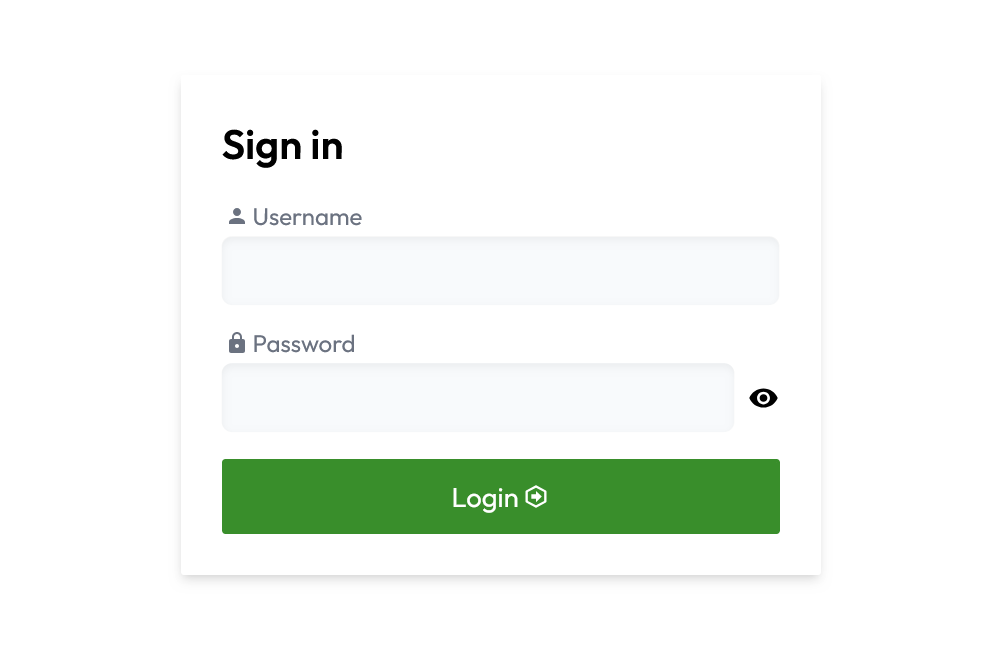
\includegraphics[width=0.8\textwidth]{img/login.png}
\caption{Layout / pagina di login}
\end{figure}

\subsection{Pagine}
Le singole pagine sono invece strutturate secondo il \emph{file-based routing} di Nuxt. In particolare, queste sono le principali pagine / rotte previste:
\begin{itemize}
    \item Login dell'utente.
    \item Homepage della dashboard, di fatto spoglia e priva di funzionalità particolari.
    \item Vista degli utenti. Nascosta a chiunque non abbia facoltà di gestione degli utenti. Permette di gestire utenti (cancellare, creare, ecc.)
    \item Vista delle task di scansione. Permette di creare task, verificare il progresso e l'esecuzione di quelli già configurati.
    \item Vista dei bersagli, da cui si possono vedere quelli già configurati e configurarne di nuovi.
    \item Viste dei risultati. Ne esistono di differenti per distinguere tra vulnerabilità vere e proprie e quelle ottenute tramite scansioni di prognosi \ref{cve}. Le viste integrano un sistema di filtraggio più avanzato e integrato rispetto alle altre strutture tabellari, siccome si presume che questa vista sarà quella su cui l'utente vorrà fare maggiori analisi.
    \item Viste dei rapporti. Di fatto fornisce un consuntivo dei risultati trovati e fornisce collegamenti ai risultati correlati e agli host determinati dalla scansione.
    \item Vista degli host. Raccoglie e visualizza degli host, con tutti i dettagli trovati organizzati nel modo più chiaro possibile.
\end{itemize}

\section{Store per QoD}
Come già detto, OpenVAS integra una stima empirica dell'affidabilità dei risultati raccolti, detta QoD. L'API realizzata espone questo parametro nelle richieste e fornendolo i risultati vengono automaticamente filtrati e restituiti solo quelli con QoD superiore al numero fornito.

Nell'interfaccia web si è deciso per avere un selettore di QoD globale, attivabile in ogni momento e la cui modifica influisce i risultati mostrati nelle pagine web. Questo si è realizzato nel concreto mediante un input range HTML, il cui valore è stato collegato tramite v-model ad una variabile di uno store Pinia.

Lo store Pinia consente di bypassare la struttura gerarchica dei componenti e di condividere globalmente la variabile del QoD ad ogni componente che ne ha bisogno.

\begin{figure}
\centering
\begin{jscode}
import { defineStore } from 'pinia'

export const useQoDStore = defineStore('qod', {
  state: () => ({ min_qod: 70, disable_input: false }),
  actions: {
    updateQoD(qod: number) {
      this.disable_input = true
      this.min_qod = qod
    },
    enableInput() {
      this.disable_input = false
    }
  }
})
\end{jscode}
\caption{Store Pinia usato per la condivisione del valore di QoD nel frontend}
\end{figure}

\section{Tipi TypeScript}
Nuxt è un framework profondamente radicato in TypeScript, per fornire type safety e altri controlli.

I tipi sono definiti in file \texttt{.d.ts}, in accordo con le convenzioni TypeScript. Di fatto sono quasi tutte interfacce TypeScript che replicano la struttura dei tipi già specificata negli schemi Marshmallow del backend.

\section{Componenti Vue}
Nuxt memorizza i componenti in una cartella \texttt{components/} gestita secondo convenzioni. In particolare, il nome delle cartelle induce automaticamente la struttura usata per effettuare import automatici dei componenti all'interno delle pagine, dei layout e di tutti gli altri componenti Vue.

Segue una spiegazione dei componenti più importanti e/o peculiari.

\subsection{Tabelle}
I componenti più importanti sono sicuramente le tabelle che organizzano e mostrano le entità. E fra questi, quello più importante è il componente generico su cui tutte le altre si basano.

\begin{figure}
\centering
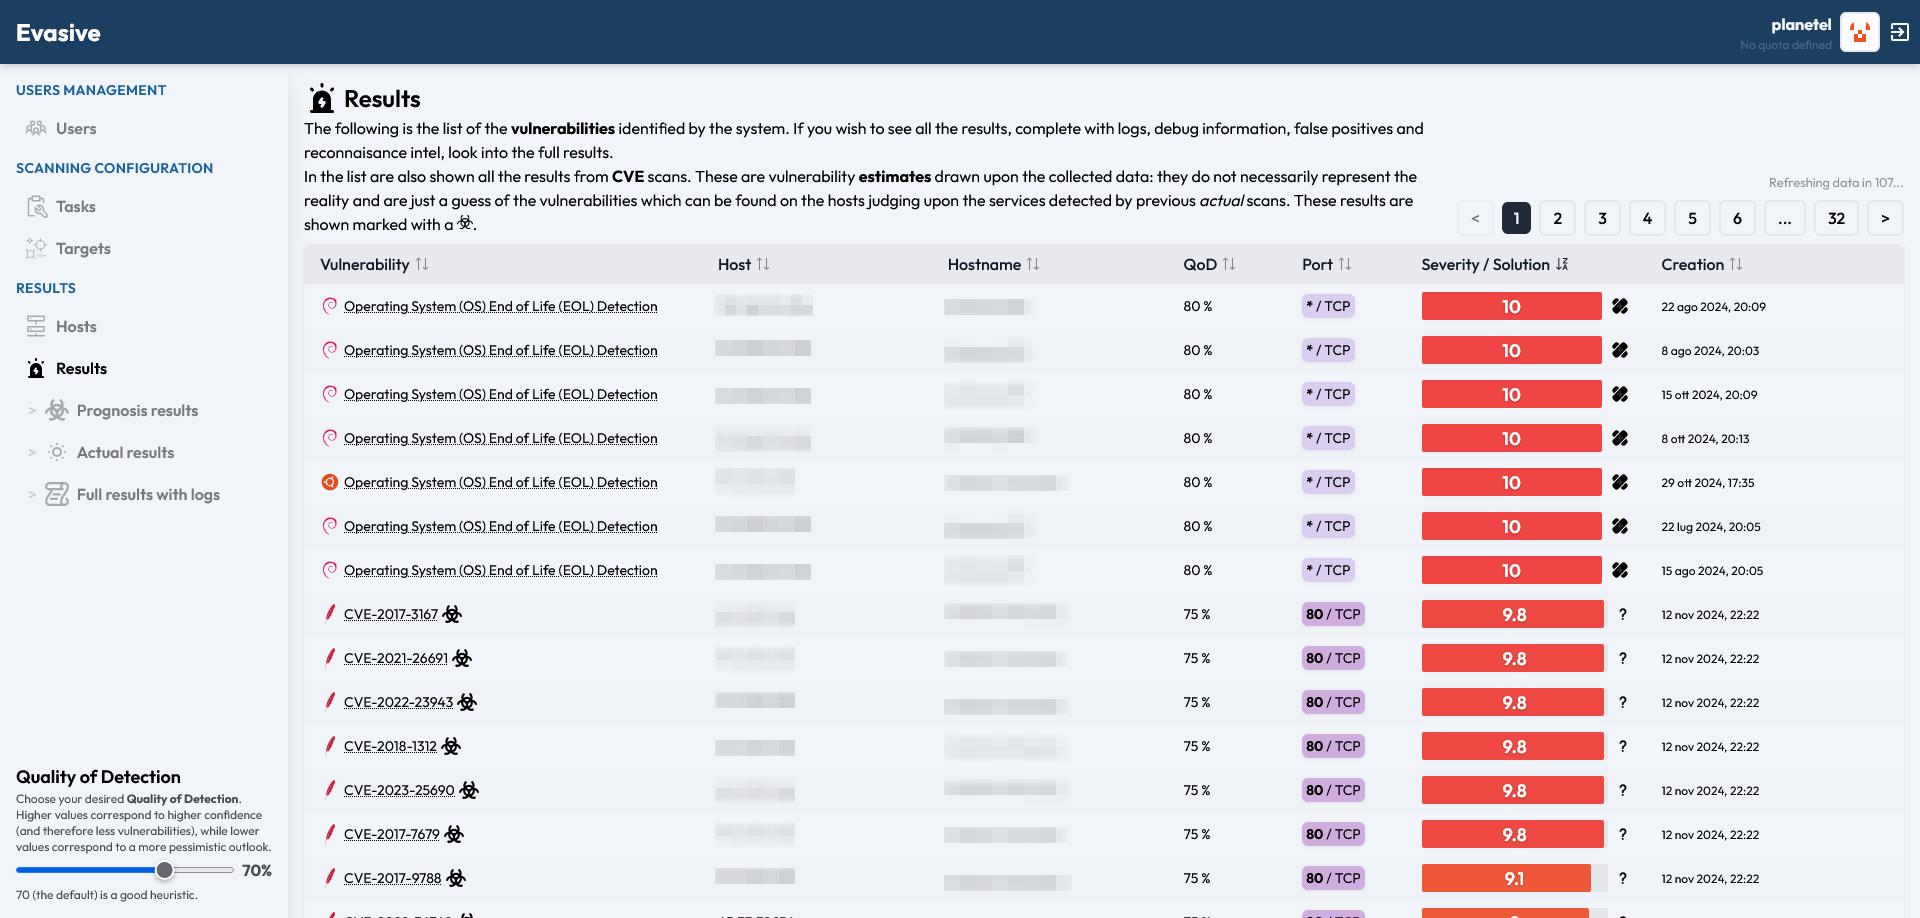
\includegraphics[width=\textwidth]{img/results.png}
\caption{Tabella dei risultati ottenuti dalle scansioni}
\end{figure}

\subsubsection{Razionale}
Di fatto il componente generico agisce come una sorta di tabella \emph{headless} che può essere configurata a seconda del caso specifico.

In questo modo si è riusciti ad avere una sorta di griglia dei dati similare come concetto a quelle fornite da librerie come Ag-Grid. Tuttavia, l'aver realizzato questo componente in autonomia consente di applicare uno stile d'aspetto specifico per il nostro progetto.

Questo comportamento è molto simile a quello che offrono librerie come Tanstack \cite{tanstack}, che forniscono componenti headless. Tuttavia, dopo un'attenta valutazione si è giunti alla conclusione che integrare librerie così avanzate sarebbe stato troppo lavoro per funzionalità aggiuntive che non si sarebbero mai usate. Inoltre, questo ha consentito di creare un'interfaccia più adatta e specifica per i nostri scopi.

\subsubsection{Funzionalità}
Il componente così creato offre le seguenti funzionalità:
\begin{itemize}
    \item Titolo, icona e altre opzioni di aspetto e contenuto sono completamente personalizzabili dagli attributi.
    \item Descrizione e azioni della tabella sono configurabili tramite \emph{named slot}. Le azioni di ogni riga sono configurabili tramite \emph{scoped slot}.
    \item Personalizzazione e scelta dell'entità che gestisce attraverso l'inserimento dell'endpoint responsabile di fornire le entità. Questo può funzionare siccome la REST API agisce in modo standardizzato per tutte le richieste indice.
    \item Reagisce ai campi di QoD.
    \item Supporta e gestisce autonomamente una paginazione di tipo server-side usando i dati forniti dal backend.
    \item Supporta il filtraggio dei dati, se dichiarato possibile dall'interfaccia.
    \item Supporta l'ordinamento \emph{server-side} delle colonne, se dichiarato possibile dalle definizioni delle colonne.
    \item \emph{Polling} dei dati ad intervalli regolari, realizzando l'aggiornamento dinamico dello stato delle scansioni, dei rapporti e dei risultati. Per questa parte è stato necessario ricorrere a \textbf{VueUse} una libreria popolare di Vue 3, che fornisce dei \emph{composable} snelli e leggeri per facilitare l'integrazione delle funzioni standard nel nuovo paradigma di Vue.
    \item Il componente gestisce in autonomia accorgimenti al frontend per gestire elegantemente gli stati di caricamento.
    \item Le righe della tabella sono animate con il componente TransitionGroup di Vue.
    \item Può mostrare un bottone il cui evento apre un modale. Il modale ha contenuto personalizzabile attraverso un Component Vue.
\end{itemize}

\subsubsection{Realizzazione}
Per realizzare il componente si sono usate varie feature di Vue e eventuali librerie aggiuntive.

La maggior parte delle opzioni del componente sono specificabili usando il meccanismo degli attributi / props, soprattutto booleani e stringhe, ma in alcuni casi anche oggetti JavaScript più strutturati:
\begin{itemize}
    \item Il componente incluso nel modale apribile dall'apposito bottone di aggiunta è specificabile tramite un Component. Siccome Nuxt usa un meccanismo di import automatico è necessario importare manualmente il componente, usando la macro \texttt{\#components} messa a disposizione da Nuxt apposta per queste situazioni.
    \item Le definizioni delle colonne, che specificano le proprietà di ognuna di essa: quale campo considerare nell'oggetto fornito, che tipo di dato è, quale \emph{renderer} usare per mostrare il dato, se la colonna è ordinabile, filtrabile e altre personalizzazioni di stile. Questo approccio è abbastanza simile a quello utilizzato da Tanstack \cite{tanstack}, sebbene più semplice e diretto.
\end{itemize}

Nel componente si è anche usata una feature di Vue abbastanza recente (3.3) ovvero i \textbf{componenti generici}. Questa funzionalità consente di definire e usare tipi generici nella funzione di \texttt{setup} del componente. Nel caso specifico si è definito un tipo generico per l'entità considerata dalla tabella.

\subsection{Renderer}
I \emph{renderer} altro non sono che un insieme di componenti dedicati a prendere un dato semplice (una stringa di caratteri, un booleano, un intero, un decimale) o strutturato (un oggetto JSON o un'array di oggetti o variabili) per poi mostrarlo all'utente in una forma \emph{user-friendly} e stilisticamente accattivante.

Nel progetto ci sono quasi 40 renderer differenti e/o innestati l'uno nell'altro, di fatto diventando una sorta di ``design pattern'' di progetto. L'uso di questo sistema porta diversi benefici:
\begin{itemize}
    \item Siccome il progetto usa un framework CSS \emph{utility-first} il segregare lo stile il più possibile in componenti atomici garantisce manutenibilità e riproducibilità.
    \item Similarmente, tanti componenti granulari garantiscono un facile riuso e quindi facile manutenibilità e ridondanza ridotta al minimo.
    \item Renderizzare anche il dato ``semplicemente'' senza ulteriori personalizzazioni fornisce un comodo livello di indirezione per aggiungere ulteriori personalizzazioni in futuro.
    \item Inoltre, renderizzare i dati in questo modo consente di realizzare personalizzazioni più avanzate che semplici modifiche stilistiche, permettendo di integrare del comportamento (apertura di modali, \emph{tooltip}, link a pagine web, ecc.)
\end{itemize}

\begin{figure}
\centering
\begin{vuesfc}
<script setup lang="ts">
import { DateTime } from 'luxon'
  
defineProps<{ value: string }>()
</script>
  
<template>
  <span v-if="value" class="text-xs truncate">
    {{ DateTime.fromISO(value).toLocaleString({month: 'short', day: 'numeric', year: 'numeric', hour: '2-digit', minute: '2-digit'}) }}
  </span>
  <span v-else />
</template>
\end{vuesfc}
\caption{Renderer usato per i timestamp, basato sulla libreria Luxon}
\end{figure}

\subsubsection{CPE}
Un renderer particolarmente interessante è quello usato per i CPE. OpenVAS infatti utilizza stringhe che rispettano il formato CPE per specificare gli \emph{asset} inventariati dalle scansioni (host e OS), ma anche l'ambiente in cui una vulnerabilità è stata rilevata.

Per rendere la consultazione dei risultati il più possibile veloce si è deciso di mostrare i CPE corredandoli di icone. Queste sono determinate a partire dai \emph{vendor} (o dai \emph{product}) specificati nella stringa CPE.

\begin{figure}
\centering
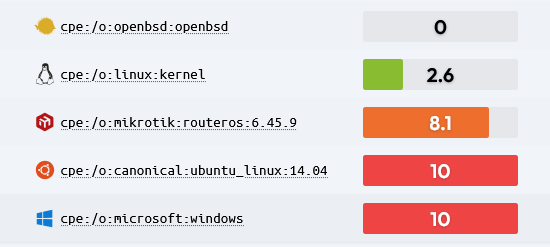
\includegraphics[width=0.6\textwidth]{img/cpe.png}
\caption{Renderer delle stringhe CPE e dei punteggi di severità}
\end{figure}

\subsubsection{Iconify}
Molti dei renderer sfruttano le icone SVG per facilitare la visualizzazione dei dati a colpo d'occhio.

Le icone sono fornite dalla libreria \textbf{Iconify} che porta in dote decine di migliaia di icone raccolte dai principali pacchetti disponibili online; queste sono poi richieste \emph{on demand} da un componente apposito (Iconify mette a disposizione un comodo wrapper per Vue).

\subsection{Modali}
I modali sono definiti tutti a partire da un componente comune, che ne fornisce le funzionalità di base. Il contenuto è personalizzabile con lo slot di default.

La caratteristica fondante di un modale è che questo in un certo senso esce dalla gerarchia del documento HTML. Questo è realizzato anche in pratica con il componente \texttt{Teleport} di Vue, che trasferisce il componente sotto il tag body.

L'apparizione del modale è animata con il componente \texttt{Transition}.

\subsection{Form}
Le form sono un altro pezzo essenziale dell'applicazione. Come in ogni progetto, la parte fondamentale e più critica di queste componenti riguarda l'inserimento e la validazione dei dati, che dev'essere il più possibile semplice e intuitivo.

\subsubsection{Validazione}
Per quanto riguarda la validazione ci si è integrati con \textbf{Vee-Validate} \cite{vee-validate}, una delle più popolari librerie di validazione \emph{client-side}. Trattandosi di validazione client-side si è badato soprattutto a fornire un \emph{feedback} veloce e informativo per l'utente. Infatti, tutti i dati sono comunque validati \emph{server-side} tramite gli schemi Marshmallow.

\subsubsection{Select e option}
Per rendere l'input dei dati il più facile possibile si è fatto largo uso del paradigma di input fornito dai tag HTML di select, ovvero i menu a discesa. In questo modo la validazione dei dati è semplificata, ma anche l'esperienza utente, che ha a disposizione un piccolo insieme di opzioni ben chiare tra cui scegliere.

Tuttavia, il componente nativo di select è piuttosto limitato:
\begin{itemize}
    \item Le opzioni permettono di avere solo testo semplice, con pochissime personalizzazioni consentite.
    \item Non esiste una possibilità di filtraggio.
\end{itemize}
Per ovviare a queste limitazioni si è fatto larghissimo uso di \texttt{vue-multiselect}, una comodissima libreria che fornisce un componente di selezione accessibile e molto personalizzabile, sia come aspetto che come comportamento.

Per ogni componente di selezione si è sfruttata questa libreria, realizzando inoltre dei componenti dedicati per il \emph{rendering} di ogni singola opzione. In questo modo, ogni componente di selezione è personalizzato appositamente per lo scopo, con icone e descrizioni, rendendo l'input dei dati particolarmente veloce e semplice.

\begin{figure}[!h]
\centering
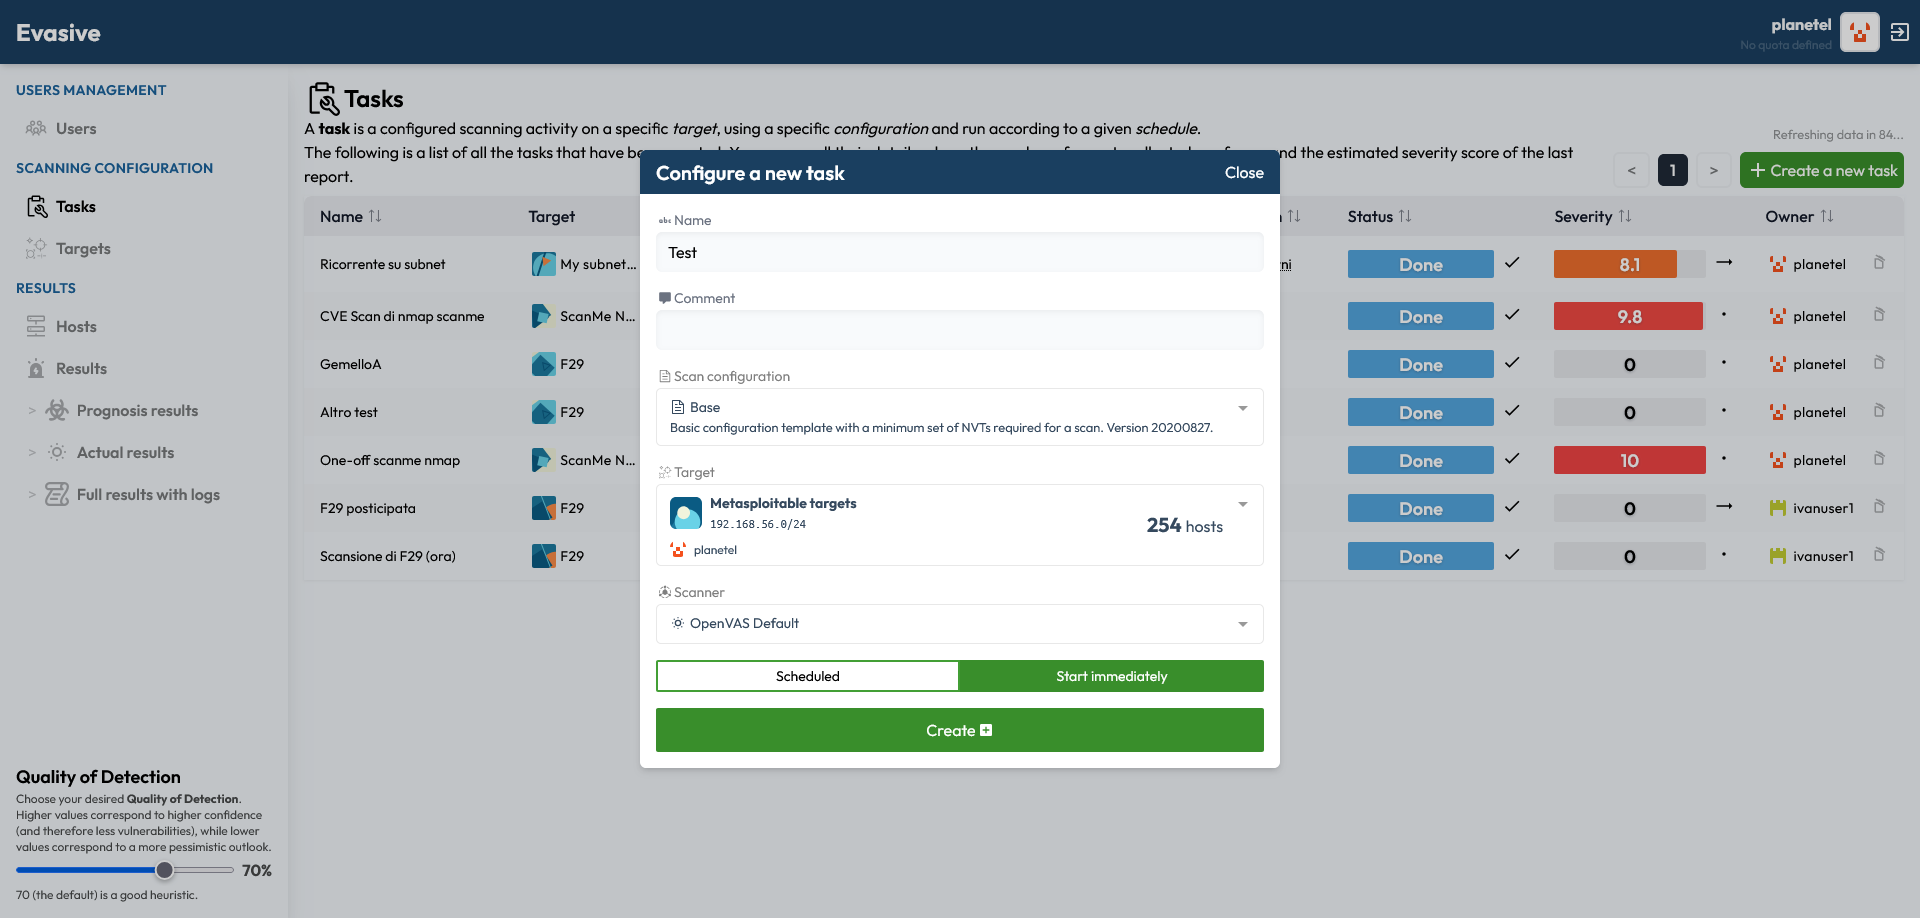
\includegraphics[width=\textwidth]{img/form-task-now.png}
\caption{Form per l'aggiunta di un nuovo task di scansione}
\end{figure}

\begin{figure}[b]
\begin{vuesfc}
<script setup lang="ts">
defineProps<{
  showModalIf: boolean;
  title: string;
}>()

defineEmits(['close'])
</script>

<template>
  <Teleport to="body">
    <Transition name="modal-fade">
      ...
    </Transition>
  </Teleport>
</template>

<style scoped>
.modal-fade-enter-from,
.modal-fade-leave-to {
  opacity: 0;
}
.modal-fade-enter-active,
.modal-fade-leave-active {
  transition: 0.25s ease all;
}
.modal-wrapper {
  position: fixed;
  left: 0;
  top: 0;
  z-index: 100;
  width: 100vw;
  height: 100vh;
  background: rgba(0, 0, 0, 0.2);
  display: grid;
  place-items: center;
}
</style>
\end{vuesfc}
\caption{Modale generico definito con i costrutti idiomatici di Vue}
\end{figure}